\section{Event Selection}
\label{sec:eventselection}

\subsection{Di-tau Candidate Selection}
\label{sec:ditauselection}
Di-tau candidates are reconstructed from muons and taus with selections described in Sections \ref{sec:muonselection} and \ref{sec:tauselection} respectively.
The muon and tau objects are required to be separated by a distance $\Delta R > 0.5$ in $\eta$-$\phi$ space to ensure that they do not represent the same physical object.

To reject background events arising from the decay of a W boson, two variables are used, the transverse mass of the $\mu$+$\met$ system ($M_{T}$), and $\pzetadiff$.
To reject this background for the MSSM Higgs search, the kinematics of tau decays is leveraged in the use of $\pzetadiff$.
In di-tau signal events the neutrinos are expected to be nearly collinear with the associated visible decay products, thus the direction of the missing transverse energy would lie between the visible decay products.
In contrast, events in which a lepton is produced via a semi-leptonic W boson decay, and to a lesser extent $t\overline{t}$ events, this correlation does not exist.
An axis $\zeta$ is defined by bisecting the directions of the visible decay products, the momentum of the visible decay products is then projected onto this axis producing the observable $p_{\zeta}^{vis}$.
An additional observable $p_{\zeta}^{miss}$ is created by projecting the missing transverse energy vector onto the same bisecting axis $\zeta$.
A final observable $\pzetadiff$ is used to reject W background events, it is defined as:
\begin{equation}
\label{eqn:pzetadiff}
\pzetadiff = p_{\zeta}^{miss} -  1.5 p_{\zeta}^{vis}
\end{equation}

In the SM search, the Higgs decays will tend to have a softer $p_{T}$ spectrum leading to the decay products being less collimated.
For this reason in order to reject this background in SM Higgs search the transverse mass is used to discriminate against events which arise from the semi-leptonic decay of a W boson.
The transverse mass is defined as 
\begin{equation}
\label{eqn:mt}
   M_{T} = p_{T}^{\mu}\met\sqrt{1-cos\Delta\phi},
\end{equation}
where $\Delta\phi$ is the angle between the muon's momentum vector and the reconstructed $\met$.
The transverse mass is required to be less than $40$ GeV.
Both the transverse mass and $\pzetadiff$ distributions can be seen in Figure \ref{fig:mtpzeta}.

\begin{figure}[ht]
  \begin{minipage}[b]{0.5\linewidth}
\centering
  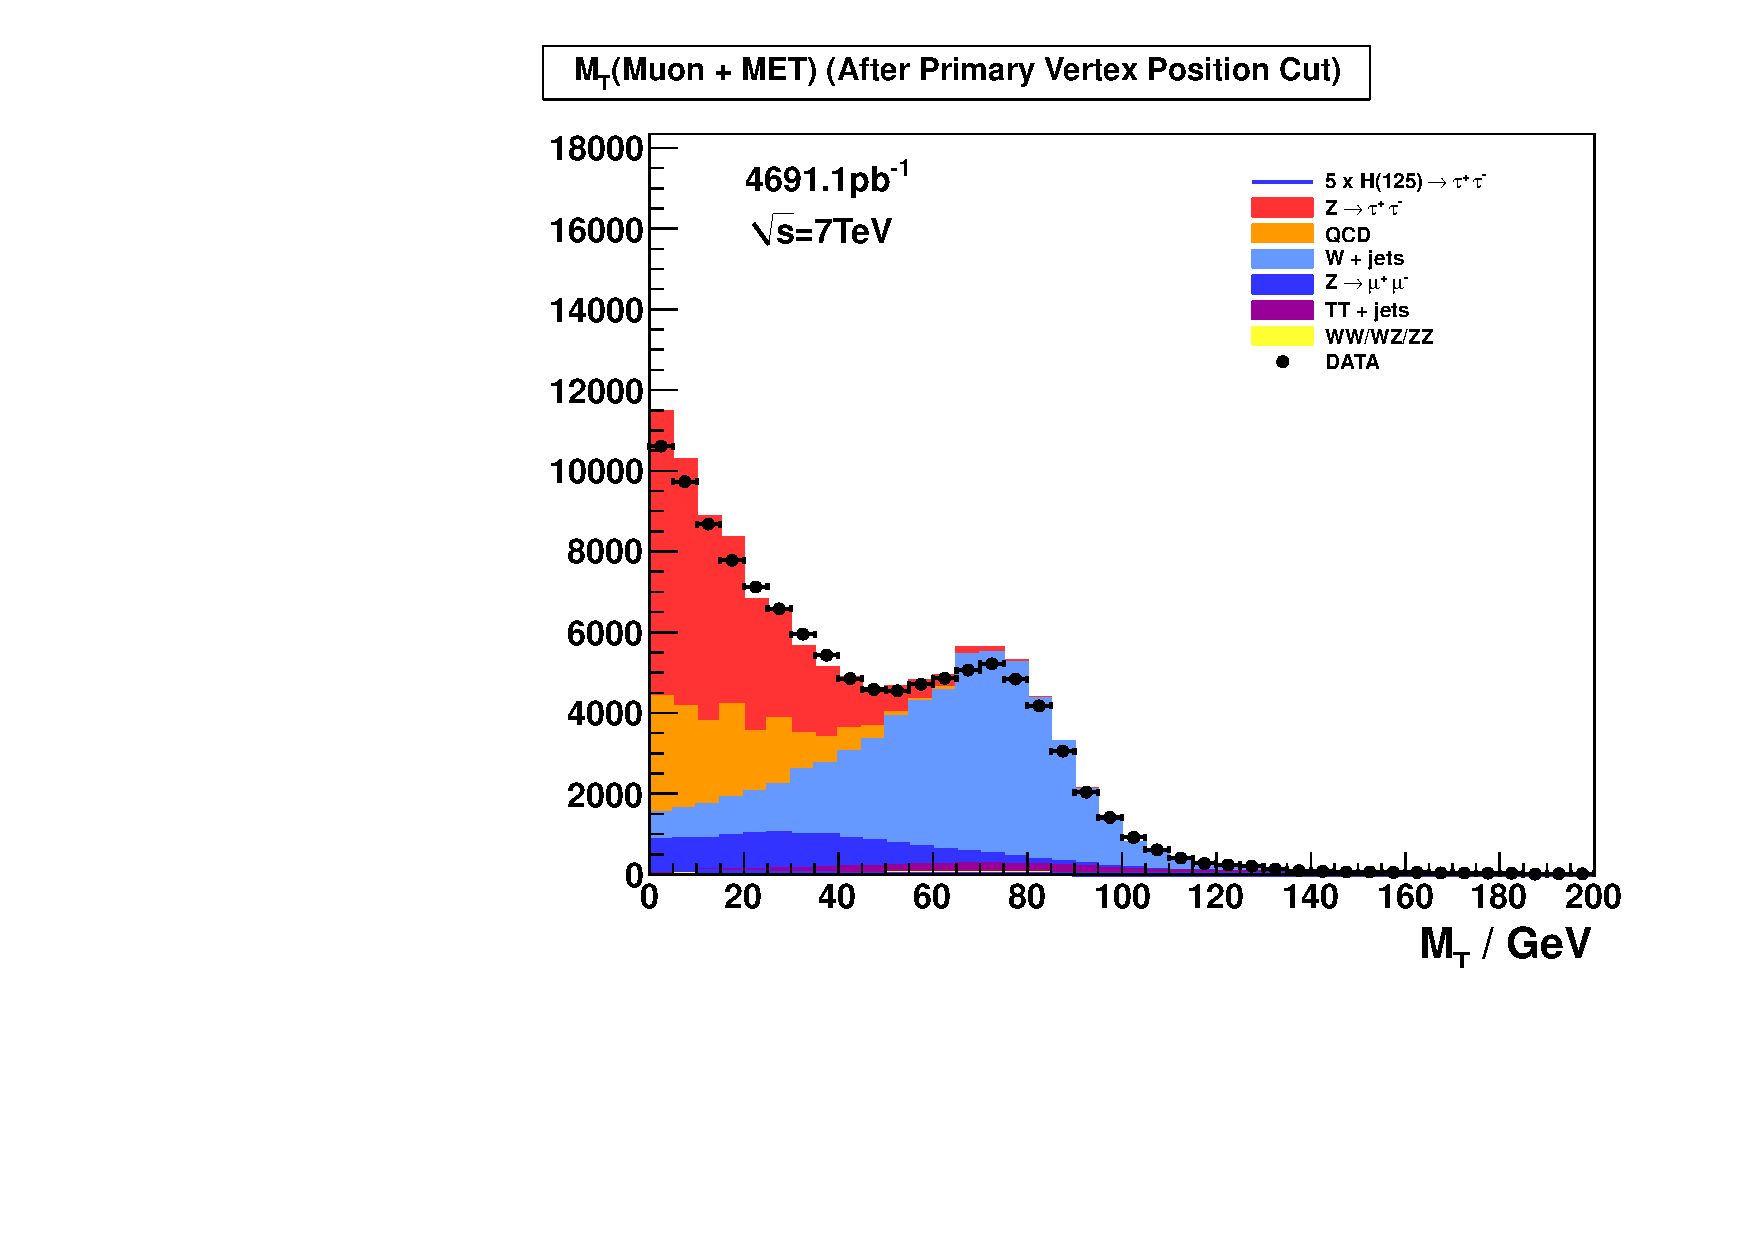
\includegraphics[scale=0.35]{plots/plotAHtoMuTau_leptonSelection_18_afterEvtSelPrimaryEventVertexPositionForMuTau_beforeEvtSelDiTauCandidateForMuTauMt1MET_mtMuonMET_linear.pdf}
\end{minipage}
\hspace{0.5cm}
\begin{minipage}[b]{0.5\linewidth}
\centering
  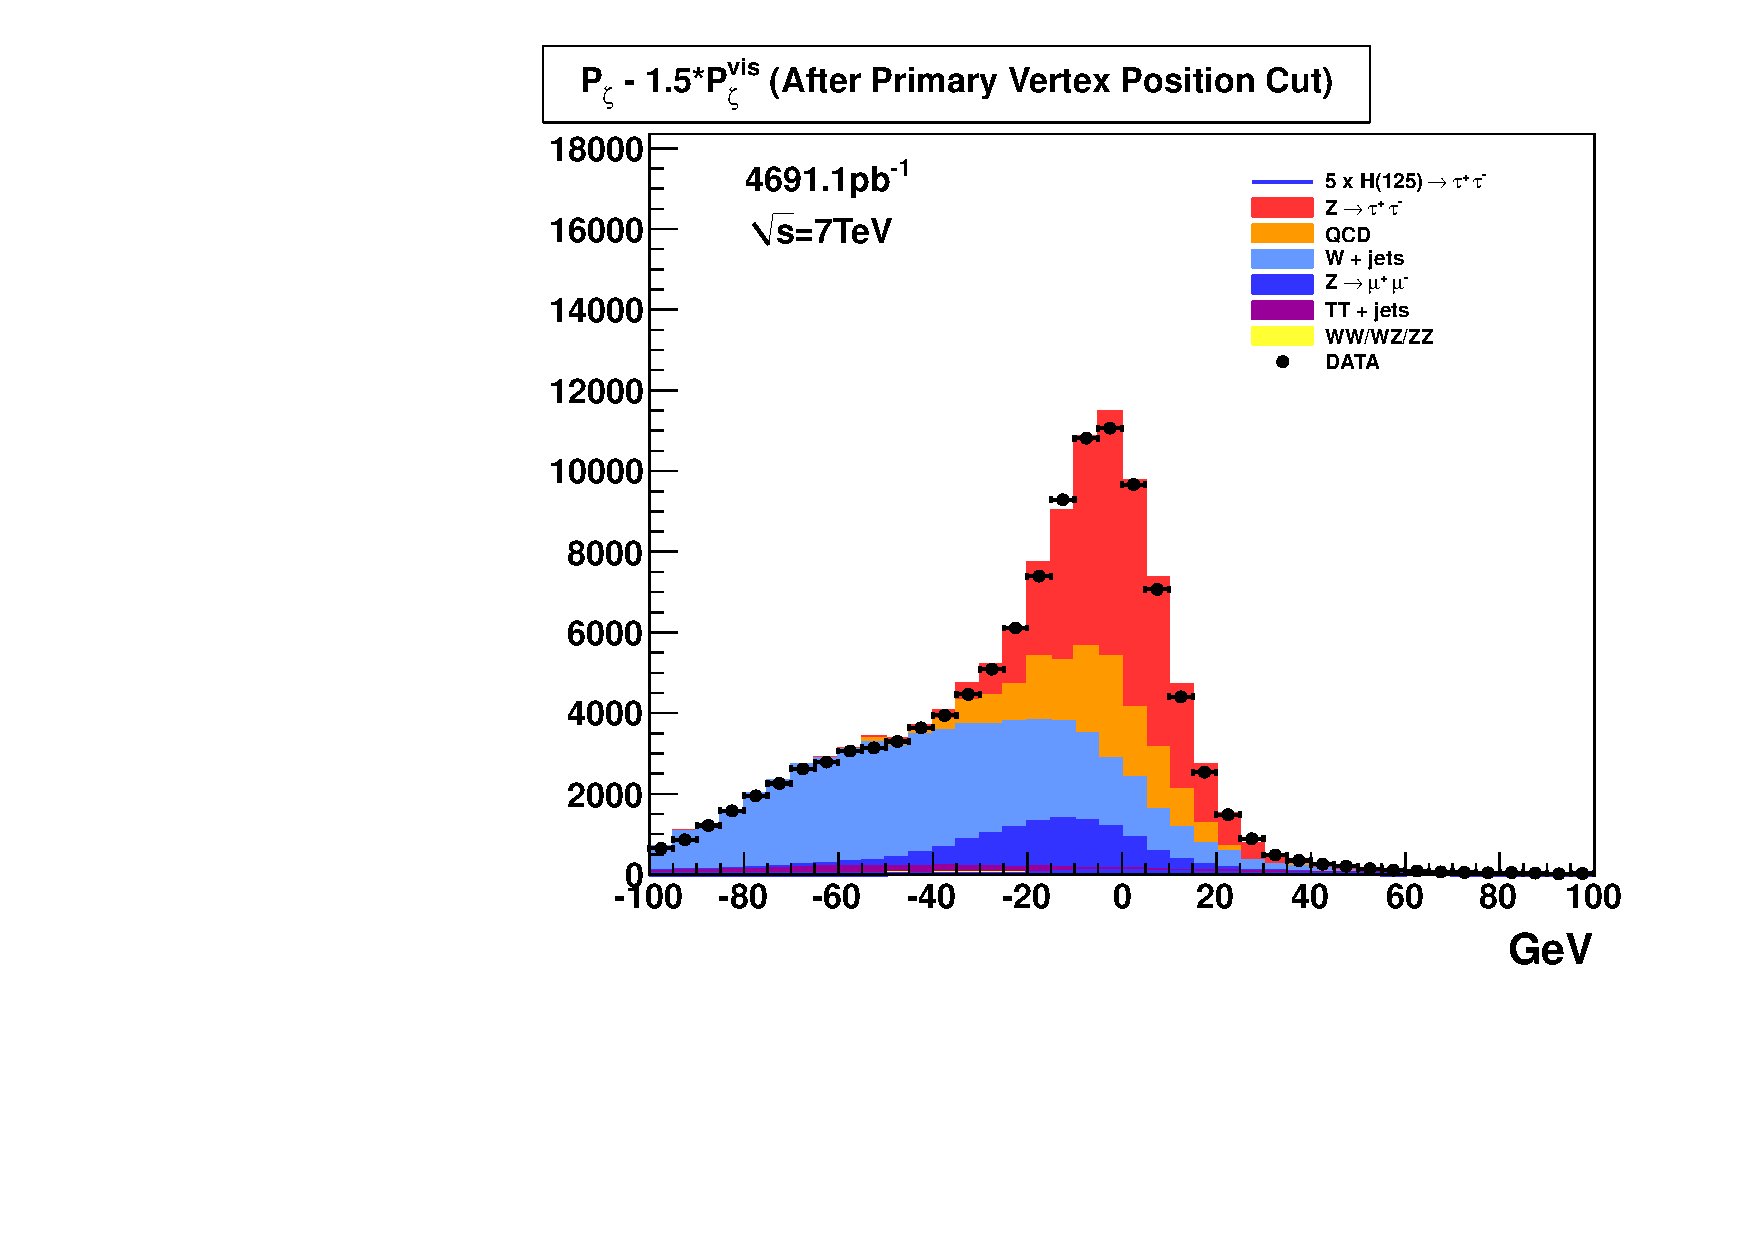
\includegraphics[scale=0.35]{plots/plotAHtoMuTau_leptonSelection_18_afterEvtSelPrimaryEventVertexPositionForMuTau_beforeEvtSelDiTauCandidateForMuTauMt1MET_PzetaDiff_linear}
\end{minipage}
\caption{$M_{T}$ and $\pzetadiff$ distributions.}
\label{fig:mtpzeta}
\end{figure}


In order to reject events arising from $Z \rightarrow \mu^{-}\mu^{+}$ an event is rejected based on the existence of a second loosely selected muon.
The second loosely selected muon is defined as a muon that has a track in the inner tracker matched to a track in the muon system, a  $p_{T} > 15$ GeV, $-2.4 < \eta < 2.4$, and $I_{rel} < 0.15$.
Once a collection of loosely selected muons is compiled the loosely selected muons are matched to muons selected as in Section \ref{sec:muonselection} using a maximum distance ($\Delta R$) in $\eta-\phi$ space of $0.5$.
An event is rejected if there are any matched muon pairs found in the event.
A similar procedure is repeated again in order to reduce backgrounds arising from the production of $Z/\gamma^{*} \rightarrow \mu^{-}\mu^{+}$.
This second di-muon rejection is performed with muons that satisfy the previous selection with the exception that the second muon does not have the $p_{T}$ and $I_{rel}$ requirements, additionally the di-muon pair is required to have zero charge and match within $\Delta R < 1.0$.


Finally since the Higgs bosons in question are neutral, a cut is applied such that the the muon and tau are required to have opposite charge.
The invariant mass of the visible tau lepton decay products before the $W$ boson discrimination, before the di-muon veto, and after the di-muon veto can be seen in Figure \ref{fig:mvisible}.
\begin{figure}[ht]
\centering
\includeditauplot{leptonSelection}{18_afterEvtSelPrimaryEventVertexPositionForMuTau_beforeEvtSelDiTauCandidateForMuTauMt1MET}{mVisible}{linear}
%\includeditauplot{leptonSelection}{18_afterEvtSelPrimaryEventVertexPositionForMuTau_beforeEvtSelDiTauCandidateForMuTauMt1MET}{mVisible}{linear}

\includeditauplot{sm}{19_afterEvtSelDiTauCandidateForMuTauMt1MET_beforeEvtSelDiMuPairZmumuHypothesisVetoByLooseIsolation}{mVisible}{linear}
%\includeditauplot{mssm}{19_afterEvtSelDiTauCandidateForMuTauPzetaDiff_beforeEvtSelDiMuPairZmumuHypothesisVetoByLooseIsolation}{mVisible}{linear}
\includefinalditauplot{zeroJets}{21_afterEvtSelDiMuPairDYmumuHypothesisVeto_beforeEvtSelJetEtCut}{mVisible}{linear}
%\includeditauplot{mssm}{21_afterEvtSelDiMuPairDYmumuHypothesisVeto_beforeEvtSelJetEtCut}{mVisible}{linear}

\caption{Invariant mass of visible tau decay products before the $W$ and $Z\rightarrow\mu\mu$ rejection (top), after the $W$ rejection (bottom left) and after the $Z\rightarrow\mu\mu$ rejection (bottom right) cuts.}
\label{fig:mvisible}
\end{figure}


\subsection{Secondary Vertex Fit}
\label{sec:nsvfit}
In order to extract the signal the invariant mass, $m_{\tau\tau}$, of the di-tau pair is fully reconstructed using a secondary vertex fit algorithm. % No Reference \cite{SVFIT}.
The algorithm performs a maximum likelihood fit taking input variables from the muon/tau four-momenta and the $\met$.
The variables to be fit for are the opening angle $\theta$ between the tau lepton and the visible momentum vector, the azimuthal angle $\overline\phi$ of the tau lepton with respect to the visible momentum vector in the laboratory frame, and the neutrino invariant mass $m_{\nu\nu}$.
The tau decay vertex (secondary vertex) is measured and an additional constraint is applied using the probability for a tau lepton to decay within the distance measured.
%(FIXME used?).
%(FIXME MORE!!!).


\subsection{Standard Model and MSSM Event Categories}
\label{sec:categories}
Events will be categorized based on the number of jets that satisfy requirements based on the jet(s) $p_{T}$, B-Tagging, and the jet(s) pseudo-rapidity.
The following standard model categories are defined according to the jet content of the event:
\begin{itemize}
\item \emph{Zero/One Jet}: This event category is designed to select events originating from the production mechanism in which the Higgs is produced via gluon-gluon fusion.
  It has the requirement that a maximum of one selected jet with $p_{T} > 30$ GeV and $-4.5 < \eta < 4.5$ is allowed.
  Secondly, in order to disallow any overlap between event categories, an event will fail to enter this category if it contains a jet with $p_{T} > 150$ GeV.
\item \emph{Boost}: This event category is designed to capture events in which the Higgs boson is highly boosted due to initial state radiation, or when produced in association with a W(Z) boson or top quark.
This category leverages the existence of a high $p_{T}$ jet recoiling from the boosted Higgs boson. 
As such the category requires a jet with $p_{T} > 150$ GeV.
%  This leads to the requirement that at least one jet must exist in the event with $p_{T} > 150$ GeV.
\item \emph{VBF}: This event category is designed to select events with the unique signature associated with vector boson fusion.
  In this category two jets with $p_{T} > 30$ GeV are required, each being located in the different hemispheres of the detector.
  Finally it is required that those jets are separated by $\Delta\eta > 4.0$ with no other selected jets between the leading jets in $\eta$.
\end{itemize}

As the MSSM Higgs has modified production mechanisms, the following categories are defined according to the jet content of the event:
\begin{itemize}
\item \emph{Non B-Tag}: This event category is designed to select events arising from the most prominent MSSM Higgs boson production mechanism of gluon-gluon fusion.
  It requires there to be no more than a single jet with $p_{T} > 30$ GeV and $-4.5 < \eta < 4.5$ while requiring zero jets with $p_{T} > 20$ GeV that meet B-Tag requirements.
\item \emph{B-Tag}: This event category is designed to leverage the MSSM Higgs boson production mechanism in association with b-quarks.
  It requires there to be no more than a single jet with $p_{T} > 30$ GeV and $-4.5 < \eta < 4.5$ while also requiring at least one jet with $p_{T} > 20$ GeV that meet B-Tag requirements.
\end{itemize}
The lepton kinematic distributions after the final event selection for \zeroJets, \boosted, \vbf, \wBtag, and \woBtag, can be seen in Figures \ref{fig:finalleptonzerojets}, \ref{fig:finalleptonboosted}, \ref{fig:finalleptonvbf}, \ref{fig:finalleptonwobtag}, and \ref{fig:finalleptonwbtag} respectively.
The reconstructed mass distribution for the SM categories \zeroJets, \boosted, and \vbf, can be seen in Figures \ref{fig:smmasszerojets}, \ref{fig:smmassboosted}, \ref{fig:smmassvbf}. 
The reconstructed mass distributions for the MSSM categories \woBtag, and \wBtag, can be seen in Figures \ref{fig:mssmmasswobtag}, and \ref{fig:mssmmasswbtag}.



% zeroJets
\begin{figure}[ht]
\includeleptonplot{zeroJets}{muon}{Pt}{log}
%\hspace{0.5cm}
\includeleptonplot{zeroJets}{tau}{Pt}{log}

\includeleptonplot{zeroJets}{muon}{Eta}{linear}
%\hspace{0.5cm}
\includeleptonplot{zeroJets}{tau}{Eta}{linear}
%
%\includeleptonplot{zeroJets}{muon}{Phi}{linear}
%\hspace{0.5cm}
%\includeleptonplot{zeroJets}{tau}{Phi}{linear}
%
\caption{Final selected $p_{T}$ (top) and $\eta$ (bottom) distributions for muons (left) and  taus (right) for the \emph{Zero/One Jets} category.}
\label{fig:finalleptonzerojets}
\end{figure}

% boosted
\begin{figure}[ht]
\includeleptonplot{boosted}{muon}{Pt}{linear}
%\hspace{0.5cm}
\includeleptonplot{boosted}{tau}{Pt}{linear}

\includeleptonplot{boosted}{muon}{Eta}{linear}
%\hspace{0.5cm}
\includeleptonplot{boosted}{tau}{Eta}{linear}
%
%\includeleptonplot{boosted}{muon}{Phi}{linear}
%\hspace{0.5cm}
%\includeleptonplot{boosted}{tau}{Phi}{linear}
%
\caption{Final selected $p_{T}$ (top) and $\eta$ (bottom) distributions for muons (left) and  taus (right) for the \emph{Boost} category.}
\label{fig:finalleptonboosted}
\end{figure}

% wVBFtag
\begin{figure}[ht]
\includeleptonplot{wVBFtag}{muon}{Pt}{linear}
\hspace{0.5cm}
\includeleptonplot{wVBFtag}{tau}{Pt}{linear}

\includeleptonplot{wVBFtag}{muon}{Eta}{linear}
%\hspace{0.5cm}
\includeleptonplot{wVBFtag}{tau}{Eta}{linear}
%
%\includeleptonplot{wVBFtag}{muon}{Phi}{linear}
%\hspace{0.5cm}
%\includeleptonplot{wVBFtag}{tau}{Phi}{linear}
%
\caption{Final selected $p_{T}$ (top) and $\eta$ (bottom) distributions for muons (left) and  taus (right) for the \emph{VBF} category.}
\label{fig:finalleptonvbf}
\end{figure}

% woBtag
\begin{figure}[ht]
\includeleptonplot{woBtag}{muon}{Pt}{log}
%\hspace{0.5cm}
\includeleptonplot{woBtag}{tau}{Pt}{log}

\includeleptonplot{woBtag}{muon}{Eta}{linear}
%\hspace{0.5cm}
\includeleptonplot{woBtag}{tau}{Eta}{linear}
%
%\includeleptonplot{woBtag}{muon}{Phi}{linear}
%\hspace{0.5cm}
%\includeleptonplot{woBtag}{tau}{Phi}{linear}
%
\caption{Final selected $p_{T}$ (top) and $\eta$ (bottom) distributions for muons (left) and  taus (right) for the \emph{Non B-Tag} category.}
\label{fig:finalleptonwobtag}
\end{figure}

% wBtag
\begin{figure}[ht]
\includeleptonplot{wBtag}{muon}{Pt}{linear}
%\hspace{0.5cm}
\includeleptonplot{wBtag}{tau}{Pt}{linear}

\includeleptonplot{wBtag}{muon}{Eta}{linear}
%\hspace{0.5cm}
\includeleptonplot{wBtag}{tau}{Eta}{linear}
%
%\includeleptonplot{wBtag}{muon}{Phi}{linear}
%\hspace{0.5cm}
%\includeleptonplot{wBtag}{tau}{Phi}{linear}
%
\caption{Final selected $p_{T}$ (top) and $\eta$ (bottom) distributions for muons (left) and  taus (right) for the \emph{B-Tag} category.}
\label{fig:finalleptonwbtag}
\end{figure}

%Mass SM
\begin{figure}[ht]
\includefullplot{zeroJets}{mSVmethod}{log}
\caption{Di-Tau invariant mass distribution in the \emph{Zero/One Jets} event category.}
\label{fig:smmasszerojets}
\end{figure}

\begin{figure}[ht]
\includefullplot{boosted}{mSVmethod}{linear}
\caption{Di-Tau invariant mass distributions in the \emph{Boost} event category.}
\label{fig:smmassboosted}
\end{figure}

\begin{figure}[ht]
\includefullplot{wVBFtag}{mSVmethod}{linear}
\caption{Di-Tau invariant mass distributions in the \emph{VBF} event category.}
\label{fig:smmassvbf}
\end{figure}

%Mass MSSM
\begin{figure}[ht]
\includefullplot{woBtag}{mSVmethod}{log}

\caption{Di-Tau invariant mass distributions in the \emph{Non B-Tag} event category.}
\label{fig:mssmmasswobtag}
\end{figure}

\begin{figure}[ht]
\includefullplot{wBtag}{mSVmethod}{linear}

\caption{Di-Tau invariant mass distributions in the \emph{B-Tag} event category.}
\label{fig:mssmmasswbtag}
\end{figure}


